% ============================================================
%  深圳大学实验报告模板(SZU Experiment Report Template)
% This template can be modified according to the specific requirements of your experiment or project.
% Produced by: Chao Fan and Kewei Ou, AI School of SZU
% ============================================================

\documentclass[a4paper,12pt]{article}

% ----------------------------
% 中文与字体支持
% ----------------------------
\usepackage{fontspec}    % 字体支持
\usepackage{xeCJK}       % 中文字体支持
\setCJKmainfont{Noto Serif CJK SC} % 设置中文字体(Overleaf自带Noto字体)

% ----------------------------
% 页面设置与常用宏包
% ----------------------------
\usepackage{geometry}    % 页面边距控制
\geometry{left=1in, right=1in, top=1in, bottom=1in}

\usepackage{longtable}   % 支持长表格
\usepackage{graphicx}    % 插入图片
\usepackage{fancyhdr}    % 页眉页脚控制
\usepackage{tikz}        % 绘制框线等图形
\usetikzlibrary{calc}    % 坐标计算
\usepackage{verbatim}    % 显示代码块
\usepackage{float}       % 控制图片浮动位置([H]参数)
\usepackage{listings}    % 代码显示
\usepackage{xcolor}      % 颜色支持

% ----------------------------
% 代码显示设置
% ----------------------------
\lstset{
    basicstyle=\ttfamily\small,
    keywordstyle=\color{blue},
    commentstyle=\color{green},
    stringstyle=\color{red},
    showstringspaces=false,
    breaklines=true,
    frame=single
}

% ----------------------------
% 页眉页脚设置
% ----------------------------
\pagestyle{fancy}
\fancyhf{} % 清空默认页眉页脚
\fancyhead[L]{深圳大学实验报告} % 左侧页眉文字
\fancyhead[C]{} % 中间空
\fancyhead[R]{} % 右侧空

% ----------------------------
% 代码显示设置
% ----------------------------
\lstset{
    keywordstyle=\color{blue},
    commentstyle=\color{green},
    stringstyle=\color{red},
    showstringspaces=false,
    breaklines=true,
    frame=single,
}

\usepackage{hyperref}
% 基本使用
\hypersetup{
    colorlinks=true,
    linkcolor=blue,
    urlcolor=cyan,
    citecolor=green,
    filecolor=magenta
}

% ============================================================
%                      文档开始
% ============================================================

\begin{document}

% ============================================================
% 封面页
% ============================================================
\begin{titlepage}
    \centering
    \vspace*{2cm}
    \Huge{\textbf{深 \ 圳 \ 大 \ 学 \ 实 \ 验 \ 报 \ 告}}\\[1.5cm]
    
    \Large{课程名称:\underline{\makebox[6cm]{Python程序设计}}}\\[0.8cm]
    \Large{项目名称:\underline{\makebox[6cm]{外星人入侵游戏改进}}}\\[0.8cm]
    \Large{学 \qquad 院:\underline{\makebox[6cm]{人工智能学院}}}\\[0.8cm]
    \Large{专 \qquad 业:\underline{\makebox[12cm]{计算机科学与技术(IEEE荣誉班)}}}\\[0.8cm]
    \Large{指导教师:\underline{\makebox[6cm]{舒婷,樊超}}}\\[0.8cm]
    \Large{报告人:\underline{\makebox[2.5cm]{姜顺元}} \quad 学号:\underline{\makebox[2.5cm]{2024401029}}}\\[0.8cm]
    \Large{实验时间:\underline{\makebox[6cm]{2025年11月25日}}}\\[0.8cm]
    \Large{提交时间:\underline{\makebox[6cm]{2025年11月26日}}}\\[2cm]

    \vfill
    \Large{教务处制}
\end{titlepage}

\newpage

% ============================================================
% 正文部分
% ============================================================

\section{实验目标 (Objectives)}

本次实验的目标是基于Github上已有代码进行功能扩展和改进。主要目标包括:

\begin{enumerate}
    \item 添加配置文件系统,使游戏设置可自定义
    \item 改进图像显示,移除图片的白色背景以支持背景颜色设置
    \item 实现玩家游戏数据的持久化存储和统计功能
    \item 添加音效和背景音乐功能,并实验性的添加了一些音效
\end{enumerate}

\section{项目概述 (Overview)}

本项目基于GitHub上代码进行功能扩展,主要改进内容包括:

\begin{enumerate}
    \item 配置文件系统 - 使用JSON格式存储游戏设置
    \item 图像处理 - 移除图片白色背景,支持自定义背景颜色
    \item 数据持久化 - 记录玩家游戏表现和统计数据
    \item 音乐和音效 - 添加了游戏的背景音乐和音效(出于版权考虑,这些素材没有上传到Github,仅保留了功能)
    \item 在Github上开发 - \href{https://github.com/ChaoFan996/Experiment-Report-Template-SZU/tree/main}{link}
\end{enumerate}

\section{实现细节 (Implementations)}

\subsection{配置文件系统}

创建了\texttt{config.json}文件来存储游戏设置,包括屏幕尺寸、飞船速度、子弹属性等:

\begin{lstlisting}[language=Python, caption=配置文件示例]
{
    "screen": {
        "width": 1200,
        "height": 800,
        "bg_color": [216, 191, 216]
    },
    "ship": {
        "speed": 1.5,
        "limit": 3
    },
    "bullet": {
        "width": 3,
        "height": 15,
        "color": [60, 60, 60],
        "speed": 25,
        "allowed": 10
    }
}
\end{lstlisting}

\subsection{数据持久化}

使用\texttt{data\_manager.py}来管理游戏数据的存储和读取:

\begin{lstlisting}[language=Python, caption=数据管理器]
class DataManager:
    def __init__(self, filename='game_data.json'):
        self.filename = filename
        self.data = self._load_data()
    
    def add_game_session(self, score, level, aliens_killed, bullets_fired, ships_left):
        # 记录游戏会话数据
        session_data = {
            "date": datetime.now().strftime(...),
            "score": score,
            "level": level,
            "aliens_killed": aliens_killed
        }
\end{lstlisting}

\section{实验结果 (Results)}

\subsection{功能测试结果}

\begin{enumerate}
    \item \textbf{配置文件功能}: 成功实现游戏设置的动态加载和保存,玩家可以自定义游戏参数
    \item \textbf{背景颜色}: 成功移除图片白色背景,支持多种背景颜色显示
    \begin{figure}[H]
        \centering
        \includegraphics[width=0.3\linewidth]{figs/imageimprove.png}
        \caption{去除背景的游戏素材图片}
        \label{fig:game-screenshot}
    \end{figure}
    \item \textbf{GUI设置界面}: 设置面板正常运行,包含速度调节、音量控制等功能
    \item \textbf{数据统计}: 游戏数据正确记录和显示,包含最高分、平均分等统计信息
\end{enumerate}

\subsection{界面展示}

\begin{figure}[H]
    \centering
    \includegraphics[width=0.3\linewidth]{figs/gamedisplay.png}
    \caption{游戏运行截图(浅紫色背景)}
    \label{fig:game-screenshot}
\end{figure}

\begin{figure}[H]
    \centering
    \includegraphics[width=0.3\linewidth]{figs/statsdisplay.png}
    \caption{统计数据界面}
    \label{fig:game-screenshot}
\end{figure}

\begin{figure}[H]
    \centering
    \includegraphics[width=0.3\linewidth]{figs/settingsdisplay.png}
    \caption{设置展示界面截图}
    \label{fig:game-screenshot}
\end{figure}

\section{讨论与分析 (Discussion)}

\subsection{技术亮点}

\begin{enumerate}
    \item \textbf{模块化设计}: 将配置管理、数据持久化、GUI界面等功能分离为独立模块
    \item \textbf{用户体验}: 通过GUI设置界面提升了游戏的可配置性和易用性
    \item \textbf{数据可视化}: 统计界面直观展示玩家游戏表现,增强游戏趣味性
\end{enumerate}

\subsection{存在问题}

\begin{enumerate}
    \item[] \textbf{已知bug}: 需要修复一些已知bug
\end{enumerate}

\subsection{总结}

本次实验实现了对外星人入侵游戏的多项功能改进。项目展示了Python在游戏开发中的应用能力,较好地完成了实验所要求的功能。同时,项目在Github上开发,使用本地的git提交代码。

\newpage

% ============================================================
% 批阅与成绩评定页
% ============================================================

% 绘制正文外框(包含批阅区域)
\begin{tikzpicture}[remember picture, overlay]
  \draw[thick] 
    ($(current page.north west)+(2cm,-3cm)$) 
    rectangle 
    ($(current page.south east)+(-2cm,2.5cm)$);
\end{tikzpicture}

\vspace{1cm}

% 批阅区
\noindent \textbf{指导教师批阅意见:}
\vspace{5cm}
\hfill

\vspace{1cm}

\noindent \textbf{成绩评定:}
\vspace{2cm}
\hfill

\vspace{1cm}

\noindent \textbf{指导教师签字:}
\vspace{2cm}
\hfill

\vspace{1cm}

% 备注部分
\noindent \textbf{备注:}
\begin{itemize}
    \item 报告内的项目或内容设置,可根据实际情况加以调整和补充。
    \item 教师批改学生实验报告时间应在学生提交实验报告时间后 10 日内。
\end{itemize}

% ============================================================
%                      文档结束
% ============================================================

\end{document}